\documentclass{article}
\usepackage{fancyhdr}
\usepackage{extramarks}
\usepackage{amsmath}
\usepackage{amsthm}
\usepackage{amsfonts}
\usepackage{tikz}
\usepackage[plain]{algorithm}
\usepackage{algpseudocode}

\begin{document}
\author{Chuan Lu}
\title{MATH:7830 Homework 2}
\maketitle


\begin{figure}[h]
\centering
\vbox{
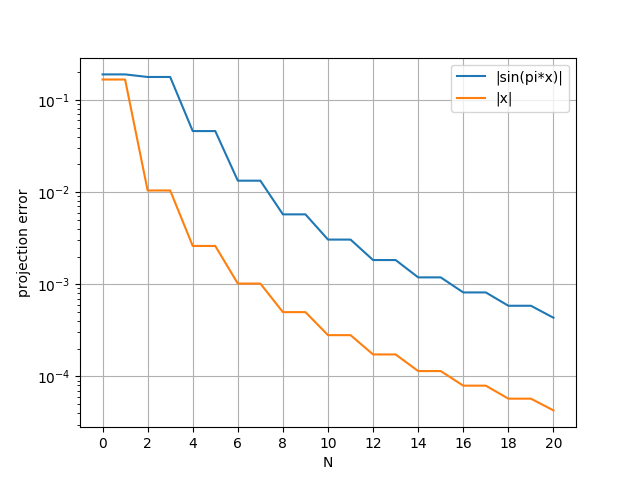
\includegraphics[scale=0.5]{Figure_1.png}
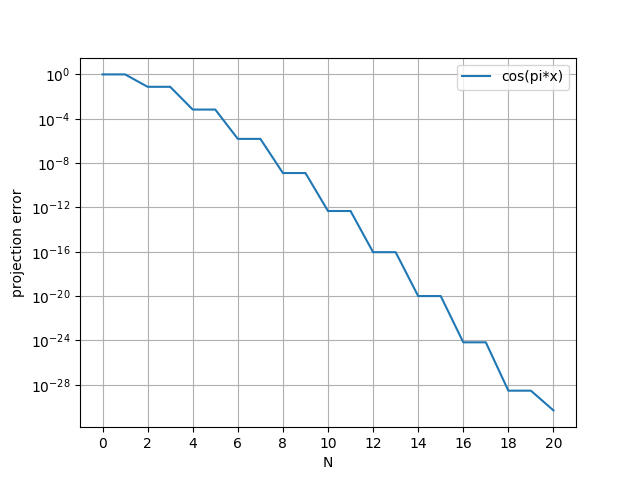
\includegraphics[scale=0.5]{Figure_2.png}
} 
\caption{The projection error of $|\sin(\pi x)|, |x|, \cos(\pi x)$ with Legendre polynomials of degree up to 20.}
\end{figure}

We notice that
\begin{enumerate}
\item The projection error for $N = 2n$ and $N = 2n+1$ are the same. This is because these three functions are even and consequently the inner product of $\phi_{2n+1} $ and $f$ equals 0.

\item The smoother the function is, the faster the convergence is. This agrees with the bound of convergence rate.

\end{enumerate}

\end{document}